\section{Evaluation} \label{sec:evaluation}
We evaluated the performance of \linksys in two main ways: \numlist{1} qualitative grading with LLM-as-a-judge and \numlist{2} pairwise preference using double-blind annotations. The first method involved using another LLM, \judgemodel, to evaluate the quality of mnemonics generated by our model, while the second involved annotators comparing mnemonics generated by the base model, \studentmodel, and our model, \linksys.

\begin{table*}[!htb]
\centering
\caption{Metric comaparison between the base (\studentmodel) and \linksys models}
\label{tab:significance-llm-judge}
\begin{tabular}{lccccc}
\toprule
\textbf{Evaluation Metric} & \textbf{Base} ($\mu$) & \linksys ($\mu$) & $\mu$ diff. & \textbf{p-value} & \textbf{Effect size} \\
\midrule
Correct vocabulary usage (bool) & 0.755 & 0.795 & +0.040 & 0.077 & -- \\
Linguistic grounding (bool) & 0.670 & 0.735 & +0.065 & \textbf{0.009} & -- \\
Association strength (1-5) & 2.845 & 3.070 & +0.225 & \textbf{<0.001} & 0.464 \\
Clarity (1-5) & 3.155 & 3.410 & +0.255 & \textbf{<0.001} & 0.481 \\
Memorability (1-5) & 2.600 & 2.900 & +0.300 & \textbf{<0.001} & 0.566 \\
\bottomrule
\end{tabular}
\begin{minipage}{\textwidth}
\vspace{0.1em}
\small
\textit{Note:} Bold p-values indicate statistically significant differences ($p < 0.05$). Effect sizes are Cohen's d, where 0.2 is small, 0.5 is medium, and 0.8 is large. Boolean metrics (first two rows) do not have effect sizes.
\end{minipage}
\end{table*}


\subsection{Qualitative grading with LLM judge} \label{sec:qualitative-llm-judge}

We designed a structured evaluation protocol using \judgemodel as a judge to assess mnemonic quality. The LLM judge evaluated 200 pairs of mnemonics from our test set, with each pair generated by the base model (\studentmodel) and our model \linksys.

We asked the judge to score each mnemonic independently on four metrics from our VAM model (\Cref{fig:good-bad-mnemonics}):
\numlist{1} whether the vocabulary is used correctly in the mnemonic,
\numlist{2} strength of association between the vocabulary and the mnemonic,
\numlist{3} how clear and easy to understand the mnemonic is,
\numlist{4} how memorable the mnemonic is, considering factors like concreteness, imageability, and distinctiveness. The last metric is \numlist{5} whether the mnemonic is linguistically grounded, meaning it incorporates linguistic features such as phonetics, morphology, or etymology.

Each criterion was evaluated on a binary scale (correct usage, linguistic grounding) or a 5-point Likert scale (association, clarity, memorability). The judge was instructed to provide six-field output: the score for each metric, and a brief reasoning for those scores.

We also calculated whether the difference in ratings was statistically significant using \numlist{1} a Wilconoxon signed-rank test for Likert ratings with paired samples and \numlist{2} a McNemar's test for paired boolean ratings. We set the significance level at 0.05.

\begin{figure}[htb]
  \centering
  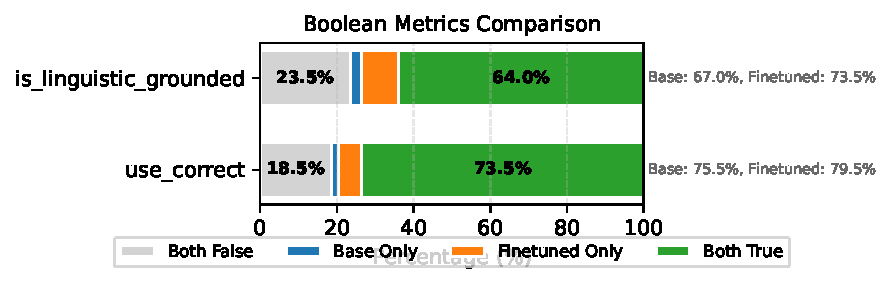
\includegraphics[width=\linewidth]{figures/boolean_comparison.pdf}
  \caption{LLM-as-a-judge evaluation for boolean metrics (true/false): correct usage of vocabulary in mnemonic and linguistic grounding of mnemonic. \linksys shows improvement in both metrics, with notable gains in linguistic grounding (68\% vs. 82\%).}
  \label{fig:llm-judge-boolean}
\end{figure}

\begin{figure}[htb]
  \centering
  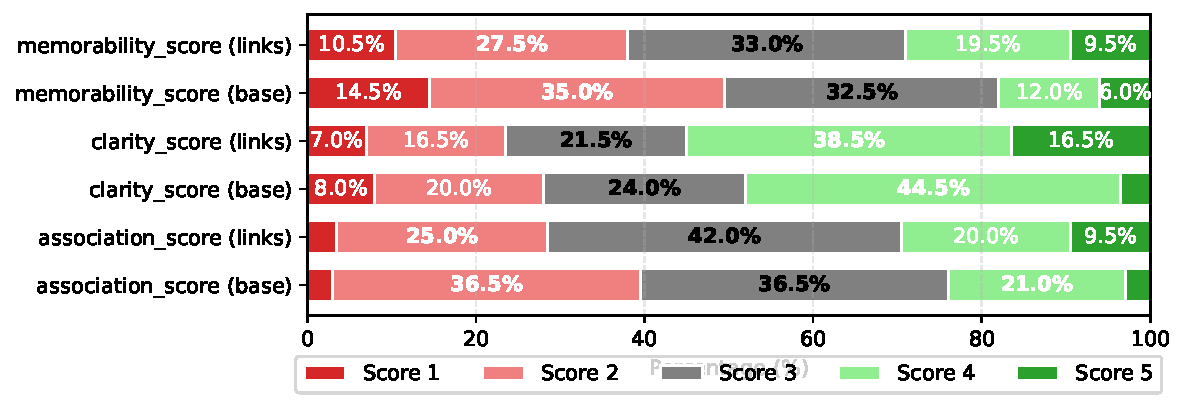
\includegraphics[width=\linewidth]{figures/likert_distribution.pdf}
  \caption{LLM-as-a-judge evaluation for 5-point Likert scale metrics. \linksys shows improvements across all three metrics, with the most significant gains in memorability (mean of 2.6 vs. 2.9)}
  \label{fig:llm-judge-likert}
\end{figure}

We reported the distribution of \judgemodel's ratings in \Cref{fig:llm-judge-boolean,fig:llm-judge-likert}, and summarized the difference in performance between the base model (\studentmodel) and our model in \Cref{tab:significance-llm-judge}. The results indicate that \linksys outperforms the base model across all evaluation metrics. Four of the five metrics showed statistically significant improvements ($p < 0.05$). The most substantial improvement was observed in memorability, with a mean difference of $+0.3$ points and a medium effect size (Cohen's $d = 0.566$). Clarity and semantic association also showed significant improvements with medium effect sizes. While correct vocabulary usage showed a positive trend, this difference was not statistically significant ($p = 0.077$). This suggests that both models were already competent at using vocabulary correctly, with less room for improvement in this area.

\subsection{Pairwise preference using double-blind annotations} \label{sec:pairwise-preference}

To further validate the quality of mnemonics generated by \linksys, we conducted a double-blind annotation study. We randomly selected 100 mnemonics from our test set, with 50 generated by the base model (\studentmodel) and 50 by our model \linksys. Two annotators were asked to evaluate the mnemonics in pairs, choosing the better mnemonic for each pair. The annotators were instructed to consider the same criteria as in the LLM-as-a-judge evaluation.

The results revealed a strong preference for mnemonics generated by our fine-tuned model over those from the base model (64\% vs. 36\%). This preference was most pronounced for abstract vocabulary terms, where linguistically grounded mnemonics provide substantial advantages over simpler associative approaches. Annotators particularly valued mnemonics that incorporated multiple linguistic features and provided clear, concrete associations to abstract concepts.

\begin{figure}[htb]
  \centering
  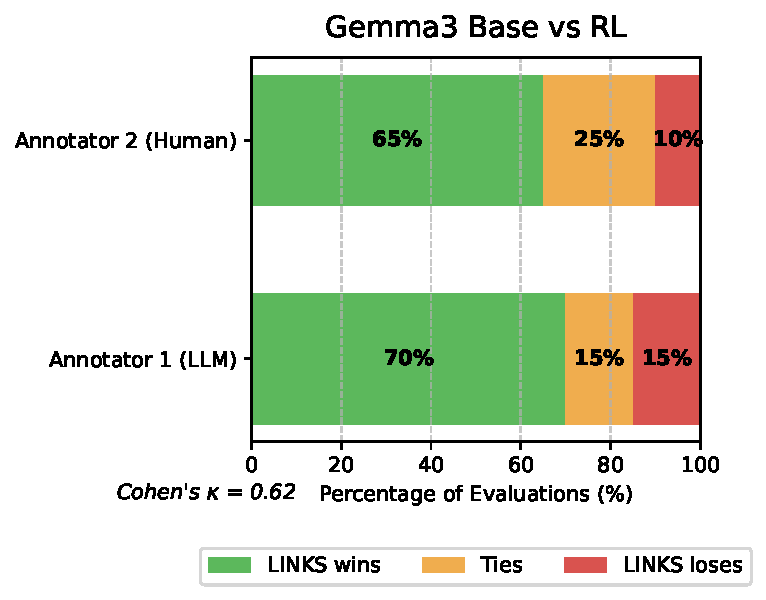
\includegraphics[width=\linewidth]{figures/model_comparison.pdf}
  \caption{Comparison of LLM-as-a-judge evaluation metrics between \studentmodel and \linksys. Y-axis shows the percentage of preference for each model.}
  \label{fig:llm-judge-comparison}
\end{figure}

We conducted a double-blind annotation study to evaluate the quality of mnemonics generated by \studentmodel and \linksys. We randomly selected 50 mnemonics from each model and presented them to annotators in pairs, asking them to choose the better mnemonic for each pair. This approach allowed us to obtain a more nuanced understanding of the relative performance of each method. In the interest of time, we only used two annotators (the author and a different LLM, \judgemodel), and noted this as a limitation in \Cref{sec:limitations}. The annotators were instructed to consider the following criteria when making their judgments:

\begin{figure}[htb]
  \centering
  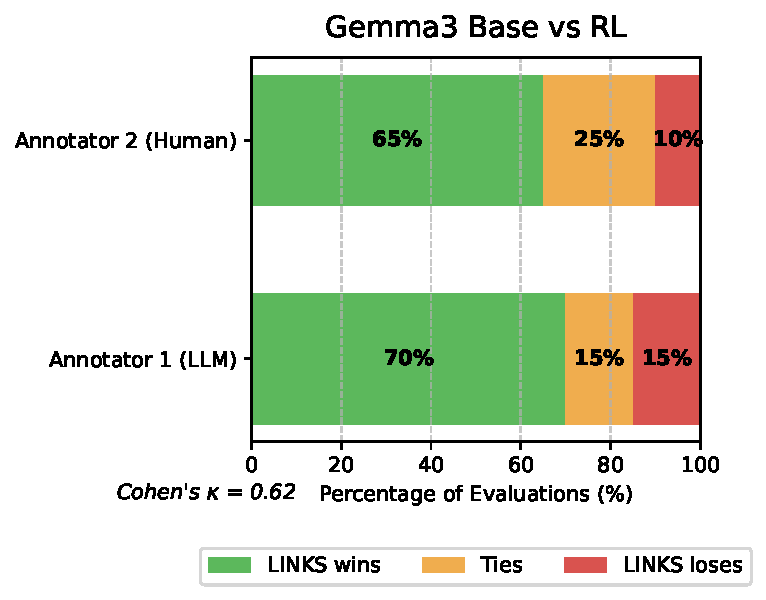
\includegraphics[width=\linewidth]{figures/model_comparison.pdf}
  \caption{Pairwise preference using double-blind annotation. Y-axis shows the percentage of preference for each mnemonic generation method.}
\end{figure}
